%!TEX TS-program = xelatex
%!TEX encoding = UTF-8 Unicode

\chapter{ผนวก ฉ.}\label{ผนวก ฉ.}

\section{แบบฟอร์ม Bird Strike Report Form ของ สำนักงานการบินพลเรือนแห่งประเทศไทย}\label{แบบฟอร์ม Bird Strike Report Form ของ สำนักงานการบินพลเรือนแห่งประเทศไทย}

\begin{figure}[ht]
\begin{center}
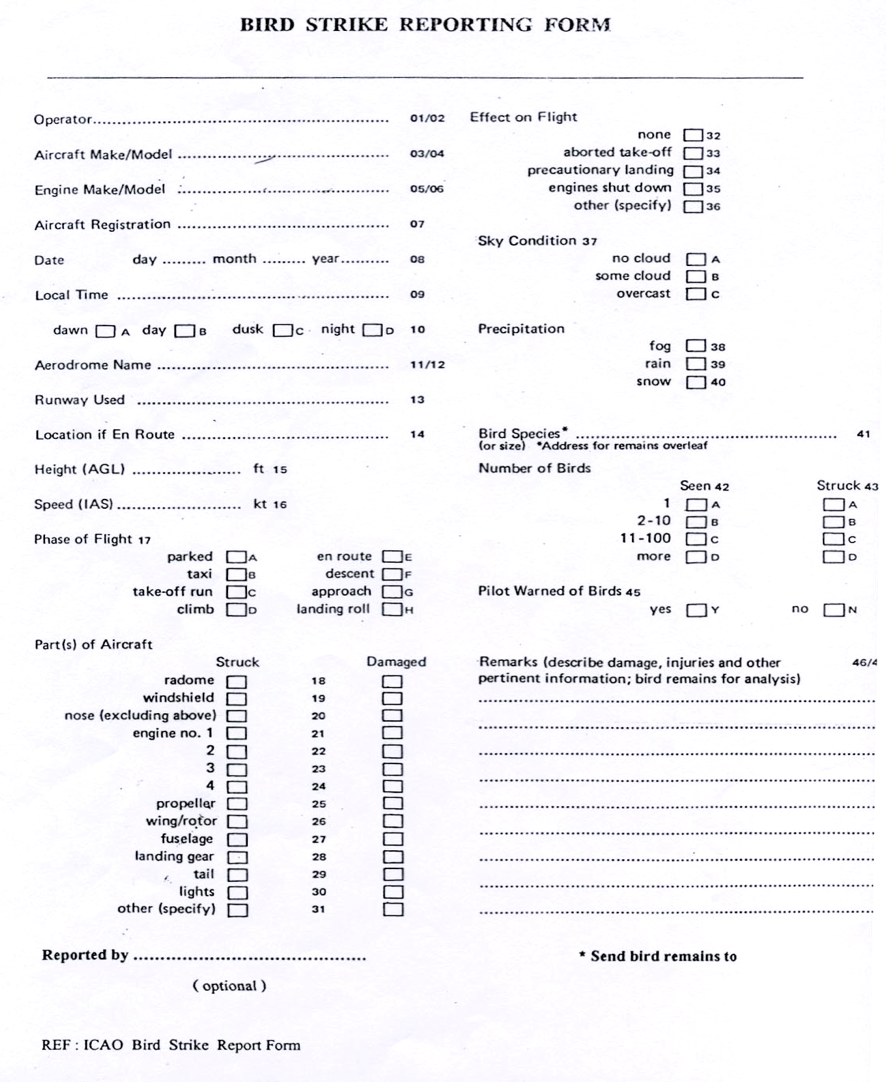
\includegraphics[width=\linewidth]{images/Bird_Strike_Report_Form.png}
\caption{Bird Strike Reporting Form}
\label{Bird Strike Reporting Form}
\end{center}
\end{figure}